\section*{Exercice 192 -- Calculs de produits vectoriels}
\setcounter{exo}{0}


\begin{center}
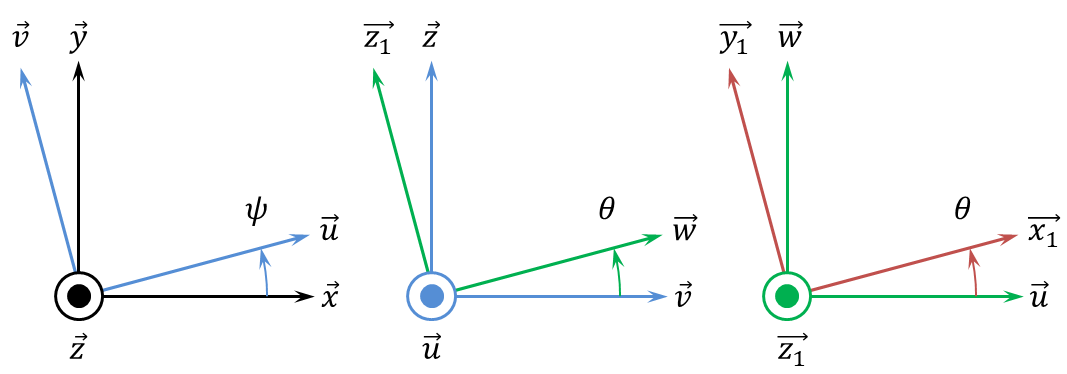
\includegraphics[width=\linewidth]{024_01}
\end{center}

Soient les produits vectoriels suivants : 
\begin{multicols}{3}
\begin{enumerate}
\item $\vect{x}\wedge\vect{y}$;
\item $\vect{v}\wedge\vect{u}$;
\item $\vect{w}\wedge\vect{v}$;
\item $\vect{y}\wedge\vect{z}$;
\item $\vect{z_1}\wedge\vect{z}$;
\item $\vect{w}\wedge\vect{u}$;
\item $\vect{x_1}\wedge\vect{w}$;
\item $\vect{y_1}\wedge\vect{u}$;
\item $\vect{z_1}\wedge\vect{u}$;
\item $\vect{x_1}\wedge\vect{v}$;
\item $\vect{x_1}\wedge\vect{z_1}$;
\item $\vect{v}\wedge\vect{y_1}$;
\item $\vect{z}\wedge\vect{z_1}$;
\item $\vect{x}\wedge\vect{y_1}$;
\item $\vect{v}\wedge\vect{x_1}$.
\end{enumerate}
\end{multicols}
\subparagraph{}
\textit{Est-il nécessaire de projeter des vecteurs pour réaliser les produits vectoriels ? Calculer les produits vectoriels.}


